\section{Reinforcement Learning}
Zunächst wird der Begriff Reinforcement Learning erklärt und von den anderen Teilgebieten des Machine Learning abgegrenzt.
Anschließend werden die zu lösenden Probleme und dafür genutzten Methoden formalisiert.

\subsection{Begriffserklärung und Abgrenzung}
\label{begriffserklaerung}
\acl{RL} (\ac{RL}) ist das Teilgebiet des \acl{ML}, das sich mit der Lösung von Entscheidungsproblemen beschäftigt \cite[S. 1]{suttonReinforcementLearningIntroduction2018}, \cite[S. 1]{vanderreeReinforcementLearningGame2013}.
\ac{RL} basiert auf der sogenannten \gqq{Reward Hypothese}, nach der jedes sequentielle Entscheidungsproblem als Optimierungsproblem beschrieben werden kann, bei dem der kumulierte Reward (\dt Belohnung) aller getroffenen Entscheidungen maximiert werden soll \cite[S. 53]{suttonReinforcementLearningIntroduction2018}, \cite[S. 24]{kontesg.SeminarReinforcementLearning2021}.

Das Ziel der \ac{RL} Methoden ist einen Agent zu trainieren, der eine Abbildung von Situationen auf die jeweils optimale Aktion lernt und so den Gesamtreward maximiert. 
Dem Agent wird nicht mitgeteilt, was die optimale Aktion in einer Situation ist. 
Stattdessen ist das grundlegende Paradigma von \ac{RL} Methoden, dass ein Agent mit seiner Umgebung interagiert und Erfahrung sammelt. 
Der Agent muss durch \gqq{trial and error} lernen, welche Aktionen in einer Situation gut sind und welche mit dem größten Reward verbunden ist. \cite[S. 1ff.]{suttonReinforcementLearningIntroduction2018}
Ein Beispiel der realen Welt sind Kinder, die laufen lernen. Dies erfolgt ohne Instruktionen, sondern nur durch \gqq{trial and error}. 
Richtige Aktionen werden belohnt durch Vorwärtskommen, während falsche Aktionen durch Fallen bestraft, \dahe negativ belohnt, werden. \cite[S. 289]{ertelIntroductionArtificialIntelligence2017}

\ac{RL} unterscheidet sich somit von den anderen Teilgebieten des \ac{ML}. Beim Supervised Learning (\dt Überwachtes Lernen) lernt ein Agent basierend auf einem gelabelten Trainingsdatensatz, die Abbildung einer Inputmenge auf einen Output. Ein Supervisor gibt dem Agenten instruktives Feedback, ob die beste Aktion gewählt wurde und was diese ist \cite[S. 289f.]{ertelIntroductionArtificialIntelligence2017}, \cite[S. 2]{suttonReinforcementLearningIntroduction2018}.

Ein \ac{RL} Agent muss hingegen seine Daten selbst durch Interaktion mit der Umgebung sammeln. 
Da der Agent seine Aktionen selbst wählt und seine Umgebung dadurch aktiv beeinflussen kann, sind die Daten stochastisch abhängig von den Aktionen, die der Agent zuvor getroffen hat. \cite[S. 16]{kontesg.SeminarReinforcementLearning2021} 
Zudem kann der \ac{RL} Agent kein instruktives Feedback erhalten, da sequenzielle Entscheidungsprobleme gelöst werden sollen und die Bewertung einzelner Aktionen gegebenenfalls nicht bekannt ist. 
Erst nach Erreichen \bzw Nicht-Erreichen des Ziels können die Aktionen bewertet und der Agent durch ein evaluatives Feedback belohnt werden. \cite[S. 17]{suttonReinforcementLearningIntroduction2018}
Dieses Problem des verzögerten Rewards ist ein weiteres Alleinstellungsmerkmal von \ac{RL} und bekannt als \gqq{Credit Assignment Problem} \cite[S. 17]{suttonReinforcementLearningIntroduction2018}.
Jedoch ermöglicht es die Anwendung von \ac{RL} auf Probleme, bei denen die optimale Strategie nicht bekannt ist. \cite[S. 2]{suttonReinforcementLearningIntroduction2018}, \cite[S. 16]{kontesg.SeminarReinforcementLearning2021}
Zudem unterscheidet sich \ac{RL} vom Unsupervised Learning (\dt Unüberwachtes Lernen).
Dieses verwendet zwar ebenfalls ungelabelte Daten, aber versucht darin Strukturen zu finden und somit andere Probleme zu lösen \cite[2]{suttonReinforcementLearningIntroduction2018}.

\subsection{Formalisierung des Reinforcement Learning Problems}
\label{formalisierung}

Eine Formalisierung des \ac{RL} Problems bedeutet eine Formalisierung der Reward Hypothese. 
Wie in \cref{begriffserklaerung} beschrieben, interagiert ein Agent mit seiner Umgebung. 
Alles außerhalb der direkten Kontrolle des Agenten wird zur Umgebung gezählt. 
Diese Trennung zwischen Agent und Umgebung wird als Agent-Umgebung-Schnittstelle bezeichnet. \cite[S. 47]{suttonReinforcementLearningIntroduction2018} 
Der Agent interagiert mit seiner Umgebung in diskreten Zeitschritten $t$. 
Man unterscheidet zwischen episodischen Problemen, die zu einem Zeitschritt $T$ enden und Problemen unendlicher Zeitdauer, die kein definiertes Ende haben \cite[S. 11]{suttonReinforcementLearningIntroduction2018}.\footnote{Probleme unendlicher Zeitdauer werden im Englischen als \gqq{continuous} bezeichnet \cite[S. 11]{suttonReinforcementLearningIntroduction2018}} 
Die Folge der Zeitschritte $t,t+1,...T$ wird als Episode bezeichnet \cite[S. 54]{suttonReinforcementLearningIntroduction2018}. 

Die Interaktion kann auf drei Signale reduziert werden, wie \cref{fig:rl_agent_environment_interaction} zeigt. 
In jedem diskreten Zeitschritt $t$ erhält der Agent den aktuellen Zustand $S_t \in S$ der Umgebung. 
Auf Basis dieser Beobachtung wählt der Agent eine Aktion $A_t \in A$. 
Im nächsten Zeitschritt erfährt der Agent, wie die Umgebung auf seine Aktion reagiert durch ein Tupel $(S_{t+1}; R_{t+1})$. 
Dies umfasst den neuen Zustand, in dem sich der Agent befindet und den Reward. 
Der letzte Zustand einer Episode $S_T$ wird als Terminalzustand bezeichnet. 
Der Reward ist definiert als $R_{t+1} \in \mathbb{R}$ und kann somit positiv oder negativ sein, um eine Belohnung und Bestrafung zu modellieren. \cite[S. 47 ff.]{suttonReinforcementLearningIntroduction2018}

\begin{figure}[h]
    \centering
    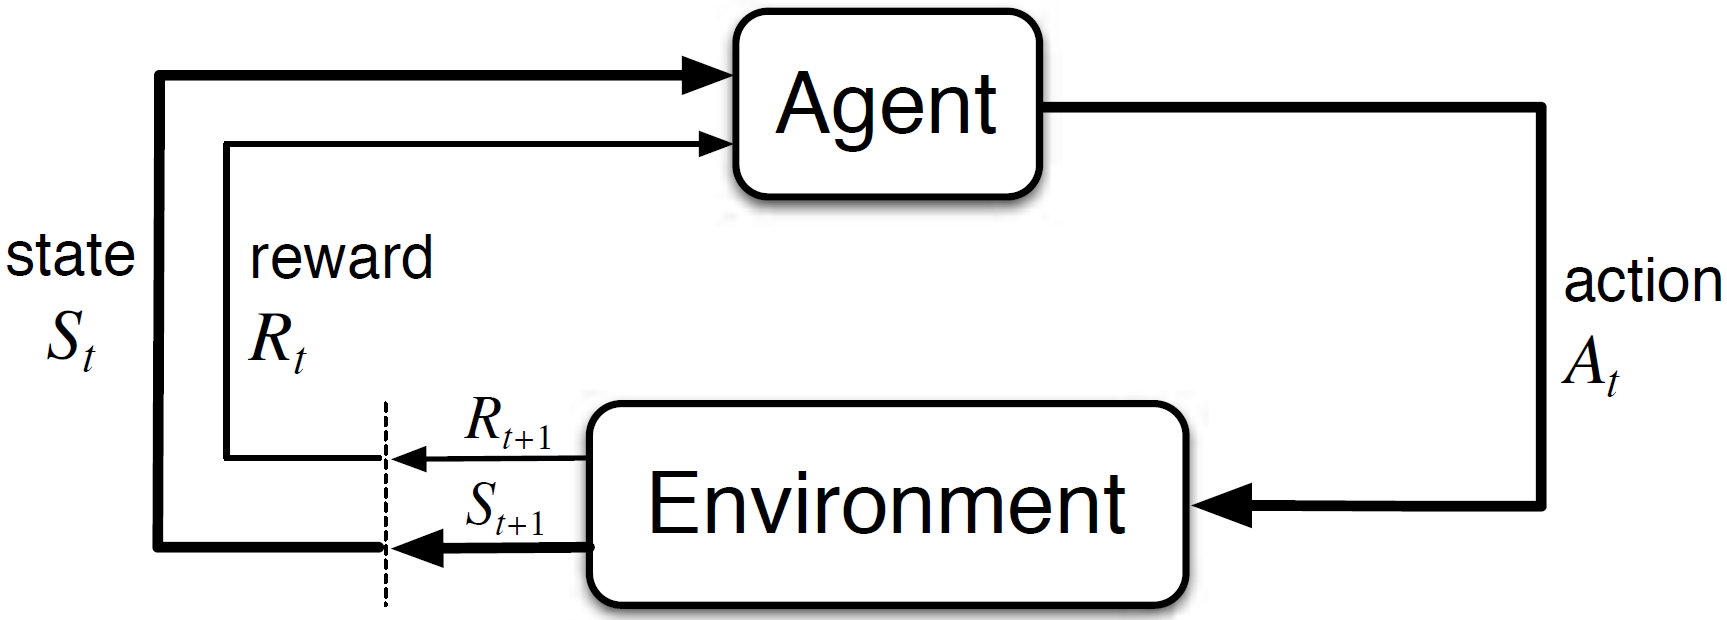
\includegraphics[scale=0.2]{04_Artefakte/01_Abbildungen/rl/rl_agent_environment_interaction.png}
    \caption[Modell der Interaktion zwischen Agent und Umgebung in einem \acs{MDP}]{Modell der Interaktion zwischen Agent und Umgebung (\engl Environment) in einem \acs{MDP} \protect\footnotemark}
    \label{fig:rl_agent_environment_interaction}
\end{figure}
\footnotetext{Abbildung entnommen aus \cite[S. 47]{suttonReinforcementLearningIntroduction2018}}

Zur Modellierung der Umgebung und deren Dynamik können \ac{MDP} genutzt werden. \ac{MDP} basieren auf  Markov Ketten und gehören zum Gebiet der mathematischen Optimierung. Ein \ac{MDP} ist definiert als ein Tupel $(S,A,p,r)$ \cite[S. 47ff.]{suttonReinforcementLearningIntroduction2018}, \cite[S. 5]{kontesg.SeminarReinforcementLearning2021}:
\begin{itemize}
    \item $S$ = Menge von Zuständen $s$
    \item $A$ = Menge möglicher Aktionen $a$
    \item $p(s' \mid s,a) = Pr(S_{t+1}=s' \mid S_{t}=s, A_{t}=a)$ für das gilt: $\sum_{a\in A}p(s'\mid s,a) =1$ \\ State-Transition Probability 
    \item $r(s,a) \rightarrow \mathbb{R}$ Rewardfunktion
\end{itemize}

Die Dynamik der Zustandsübergänge wird modelliert durch die State-Transition Probability $p$ (\dt Zustandsübergangs Wahrscheinlichkeit). 
Sie beschreibt die Wahrscheinlichkeit, bei Wahl von Aktion $a$ im Zustand $s$ in den Folgezustand $s'$ überzugehen.
Die State-Transition Probability ist als Wahrscheinlichkeitsverteilung definiert, da die Zustandsübergänge nicht deterministisch sein können. 
%Die Wahl von Aktion $a$ in Zustand $s$ kann in unterschiedlichen Folgezuständen $s'$ resultieren. 
%Die einzige Ausnahme sind Terminalzustände $S_T$, die per Definition ihr eigener Folgezustand sind \cite[S. S. 47]{suttonReinforcementLearningIntroduction2018}: $p(s \mid s,a)=1, \forall a \in A \mid S_T =s$

Zudem definiert die State-Transition Probability, dass der Folgezustand $s'$ nur vom Zustands $s$ und der darin gewählten Aktion $a$ abhängig ist. 
Zuvor besuchte Zustände oder gewählte Aktionen müssen zur Berechnung des Folgezustands nicht bekannt sein und sind implizit im Zustand $s$ enthalten. Dies wird als Markov Eigenschaft bezeichnet und ist Voraussetzung dafür, dass ein Problem als ein \ac{MDP} formuliert werden kann. \cite[S. 66]{suttonLearningPredictMethods1988}

Nach jeder Aktion des Agenten verteilt die Umgebung abhängig vom aktuellen Zustand einen Reward gemäß der Rewardfunktion. 
Die Rewardfunktion definiert das Ziel, das der Agent erreichen soll, da dieser den kumulierten Reward maximiert.
Der kumulierte Reward, den der Agent ausgehend vom Zeitschritt $t$ erhält, wird als Return $G_t$ bezeichnet. 
Für episodische Probleme ist der Return definiert als \cite[S. 54]{suttonReinforcementLearningIntroduction2018}:

\begin{equation}
    \label{eq:return_episodic}
    \equationentry{Berechnung Return $G_t$ für episodische Probleme}
    G_t=R_{t+1}+R_{t+2}+...+R_T
\end{equation}

Für Markov-Prozesse mit einer unendlichen Dauer. \dahe eine diskrete, unendliche Markov-Kette, ist $G_t$ eine unendliche Reihe, für die zur Berechnung ein Diskontierungsfaktor  $0 \le \gamma \le 1$ notwendig ist
Der Diskontierungfaktor kann auch auf episodische Probleme angewandt werden, um das Verhalten des Agenten zu beeinflussen. 
Für $\gamma=0$ beträgt $G_t= R_{t+1}$, sodass der Agent nur den direkten Reward maximiert. 
Hingegen beachtet der Agenten die späteren Rewards mit steigendem $\gamma$ mehr. \cite[S. 55f.]{suttonReinforcementLearningIntroduction2018}

\begin{equation}
    \label{eq:return_continuous}
    \equationentry{Berechnung Return $G_t$ für Probleme unendlicher Zeitdauer}
    G_t=R_{t+1}+\gamma R_{t+2}+\gamma^2R_{t+3} + \dots =\sum_{k=0}^{\infty}\gamma^{k}R_{t+k+1}
\end{equation}

Da ein Return $G_t$ den darauf folgenden Return $G_{t+1}$ enthält, kann \cref{eq:return_continuous} umgeformt werden in \cref{eq:return_nextstate}, um diese Beziehung zu verdeutlichen. Diese Beziehung aufeinander folgender Returns ist die Basis vieler \ac{RL} Methoden. \cite[S. 54 f.]{suttonReinforcementLearningIntroduction2018}

\begin{equation}
    \label{eq:return_nextstate}
    \equationentry{Beziehung aufeinander folgender Returns}
     G_t= R_{t+1}+\gamma R_{t+2}+\gamma^2R_{t+3} +\dots = R_{t+1}+\gamma(R_{t+2}+\gamma R_{t+3} +  \dots) = R_{t+1}+\gamma G_{t+1}
\end{equation}

 
Ein Beispiel für ein \ac{RL} Problem, das als \ac{MDP} modelliert werden kann, ist die sogenannte \gqq{Gridworld} in \cref{fig:gridworld_blank}. 
Der Agent startet im Feld $C1$ und soll lernen das Feld A4 zu erreichen. 
Der Zustandsraum sind die einzelnen Felder, die der Agent betreten kann. 
Das Feld B2 repräsentiert ein Hindernis und zählt nicht zum Zustandsraum. 
Die Felder A4 und B4 sind Terminalzustände. 
In jedem Zustand wählt der Agent als Aktion eine Himmelsrichtung, in der er sich bewegen möchte. Somit umfasst der Aktionsraum für jeden Zustand: Norden, Westen, Süden und Osten. 
Bei einer Bewegung in Richtung Wand oder dem Hindernis B2 verbleibt der Agent im gleichen Feld. 
Die Zustandsübergänge sind nicht deterministisch. 
Wählt der Agent eine Richtung aus, bewegt er sich nur mit einer Wahrscheinlichkeit von 80\% dorthin. 
Es besteht eine Wahrscheinlichkeit von je 10\%, dass sich der Agent in eine der angrenzenden Richtungen bewegt. 
Die Rewardfunktion definiert das Ziel des Agenten. 
Erreicht der Agent das Feld A4 erhält er einen Reward von $+1$. 
Hingegen erhält er im Agent beim Erreichen des Feldes B4 eine Bestrafung von $-1$. 
Der direkt Reward für jeden anderen Zustandsübergang des Agenten beträgt $-0,1$.
Da der Agent den Return maximiert, versucht er dadurch das Ziel in möglichst wenigen Zustandsübergängen zu erreichen. \cite[S. 10 ff.]{kontesg.SeminarReinforcementLearning2021}

\begin{figure}
    \centering
    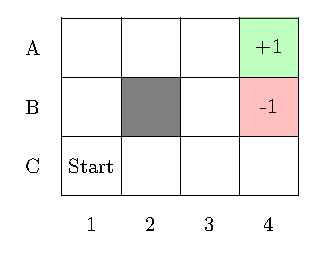
\includegraphics{gridworld/gridworld_blank.pdf}
    \caption[Aufbau des \gqq{Gridworld} Problems]{Aufbau des \gqq{Gridworld} Problems. Agent startet im Feld C1. Die Felder A4 und B4 sind Terminalzustände. B2 ist ein Hindernis.\protect\footnotemark}
    \label{fig:gridworld_blank}
\end{figure}
\footnotetext{eigene Darstellung in Anlehnung an \cite[S. 10ff.]{kontesg.SeminarReinforcementLearning2021}}

\subsection{Policy und State-Value Funktion}
\label{sec:policy_statevalue}

Der Return $G_t$ ist abhängig von den Aktionen, die der Agent in jedem Zustand wählt. 
Die Strategie, nach der Aktionen gewählt werden, wird als Policy $\pi$ bezeichnet.
Eine Policy $\pi$ ist eine Funktion $\pi(a \mid s)$, die für alle Zustände $s \in S$ die Wahrscheinlichkeit definiert, dass der Agent eine Aktion $a \in A$ wählt. 
Somit beschreibt eine Policy das Verhalten eines Agenten in jedem Zustand. 
Eine Policy kann stochastisch $\pi(a \mid s)$ oder deterministisch $\pi (s)$ sein. \cite[S. 58]{suttonReinforcementLearningIntroduction2018}

Auf der Basis einer Policy kann jedem Zustand ein Wert zugewiesen werden, der als State-Value (\dt Zustandswert) bezeichnet wird. 
Der State-Value ist der Erwartungswert des Return $G_t$, wenn der Agent im Zustand $s$ der Policy $\pi$ bis zum Ende der Episode folgt. 
Diese Abbildung von Zustand auf State-Value ist die State-Value Funktion:

\begin{equation}
    \label{eq:statevalue_function}
    \equationentry{Definition State-Value Funktion}
    v_{\pi}(s)=\mathbb{E}[G_t|S_t=s]
\end{equation}

Die State-Value Funktion kann mittels \cref{eq:return_nextstate} als Return aufeinander folgender Zeitschritte und somit aufeinander folgender State-Value Funktionen umgeformt werden:

\begin{equation}
    \label{eq:statevalue_relation}
    \equationentry{Beziehung zwischen State-Value Funktionen aufeinander folgender Zeitschritte}
    v_{\pi}(s)=\mathbb{E}_\pi[G_t|S_t=s] = \mathbb{E}_\pi[R_{t+1}+\gamma G_{t+1}]= R_{t+1} + \gamma \mathbb{E}[G_{t+1} \mid S_{t+1}=s']=R_{t+1}+v_\pi(s')
\end{equation}

\cref{fig:gridworld_policy_statevalue} zeigt für das Beispiel Gridworld eine mögliche deterministische Policy und die dazugehörige Zuweisung von State-Values. Ein Pfeil symbolisiert die Aktion, die der Agent gemäß Policy im jedem Zustand wählt. Zur Berechnung der State-Values wurde die oben beschriebene Rewardfunktion und ein Diskontierungsfaktor $\gamma=0,9$ verwendet.


\begin{figure}
    \centering
    \begin{subfigure}[b]{0.45\textwidth}
      \centering
      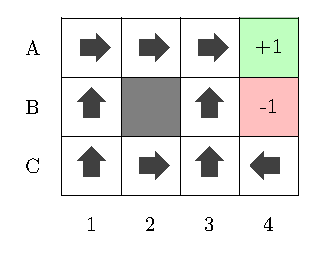
\includegraphics[]{gridworld/gridworld_policy.pdf}
      \caption{Mögliche Policy $\pi$}
      \label{fig:gridworld_policy}
    \end{subfigure}
    \begin{subfigure}[b]{0.45\textwidth}
      \centering
      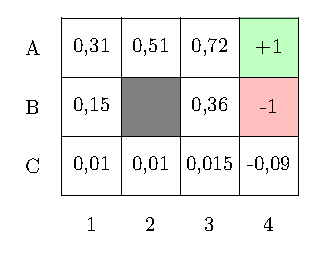
\includegraphics[]{gridworld/gridworld_statevalues.pdf}
      \caption{State-Values zur Policy $\pi$ aus (a)}
      \label{fig:gridworld_statevalues}
    \end{subfigure}
    \caption[Policy und State-Value für das Beispiel Gridworld]{Policy und State-Value für das Beispiel Gridworld\protect\footnotemark}
    \label{fig:gridworld_policy_statevalue}
    
\end{figure}
\footnotetext{eigene Darstellung in Anlehnung an \cite[S. 75.]{kontesg.SeminarReinforcementLearning2021}}

Die State-Value Funktion ermöglicht den Vergleich von Policies.
Eine Policy $\pi$ ist besser als eine andere Policy $\pi'$ wenn ihre zugehörige State-Value Funktion für alle Zustände $s$ einen größeren Wert hat, als die Policy $\pi'$: $v_\pi(s) \ge v_{\pi'}(s) \forall s \in S$

Es kann mindestens eine Policy geben, die besser als alle anderen Policies oder gleich gut ist.
Diese Policy wird als optimale Policy $\pi_*$ bezeichnet und die zugehörige Value Funktion als optimale State-Value Funktion $v_*$. \cite[S. 61 ff.]{suttonReinforcementLearningIntroduction2018}
Eine Policy ist optimal, wenn der Return $G_t$ für jeden Zustand $s \in S$ den maximal möglichen Wert annimmt.
Somit ist die optimale Policy $\pi_*$ die Lösung für den \ac{MDP} und das darin formulierte \ac{RL} Problem \cite[S. 62 ff.]{suttonReinforcementLearningIntroduction2018}.
Ist für einen \ac{MDP} das Tupel $(S,A,p,r)$ gegeben, kann die optimale Policy durch Dynamic Programming ermittelt werden. Beim Dynamic Programming wird ein Gleichungssystem aufgestellt und durch iteratives Verbessern der Policy und State-Value Funktion gelöst.\cite[S. 73ff.]{suttonReinforcementLearningIntroduction2018} 